\documentclass[
	a4paper,
	oneside,
	BCOR = 10mm,
	DIV = 12,
	12pt,
	headings = normal,
]{scrartcl}

%%% Length calculations
\usepackage{calc}
%%%

%%% Support for color
\usepackage{xcolor}
\definecolor{lightblue}{HTML}{03A9F4}
\definecolor{red}{HTML}{F44336}
%%%

%%% Including graphics
\usepackage{graphicx}
%%%

%%% Font selection
\usepackage{fontspec}

\setromanfont{STIX Two Text}[
	SmallCapsFeatures = {LetterSpace = 8},
]

\setsansfont{IBM Plex Sans}[
	Scale = MatchUppercase,
]

\setmonofont{IBM Plex Mono}[
	Scale = MatchUppercase,
]
%%%

%%% Math typesetting
\usepackage{amsmath}

\usepackage{unicode-math}
\setmathfont{STIX Two Math}
%%%

%%% List settings
\usepackage{enumitem}
\setlist[enumerate]{
	label*      = {\arabic*.},
	leftmargin  = *,
	labelindent = \parindent,
	topsep      = 1\baselineskip,
	parsep      = 0\baselineskip,
	itemsep     = 1\baselineskip,
}

\setlist[itemize]{
	label*      = {—},
	leftmargin  = *,
	labelindent = \parindent,
	topsep      = 1\baselineskip,
	parsep      = 0\baselineskip,
	itemsep     = 1\baselineskip,
}

\setlist[description]{
	font        = {\rmfamily\upshape\bfseries},
	topsep      = 1\baselineskip,
	parsep      = 0\baselineskip,
	itemsep     = 0\baselineskip,
}

%%%

%%% Structural elements typesetting
\setkomafont{pagenumber}{\rmfamily}
\setkomafont{disposition}{\rmfamily\bfseries}

% Sectioning
\RedeclareSectionCommand[
	beforeskip = -1\baselineskip,
	afterskip  = 1\baselineskip,
	font       = {\normalsize\bfseries\scshape},
]{section}

\RedeclareSectionCommand[
	beforeskip = -1\baselineskip,
	afterskip  = 1\baselineskip,
	font       = {\normalsize\bfseries\itshape},
]{subsection}

\RedeclareSectionCommand[
	beforeskip = -1\baselineskip,
	afterskip  = 1\baselineskip,
	font       = {\normalsize\bfseries},
]{subsubsection}

\RedeclareSectionCommand[
	beforeskip = -1\baselineskip,
	afterskip  = -0.5em,
	font       = {\normalsize\mdseries\scshape\addfontfeatures{Letters = {UppercaseSmallCaps}}},
]{paragraph}
%%%

%%% Typographic enhancements
\usepackage{microtype}
%%%

%%% Language-specific settings
\usepackage{polyglossia}
\setmainlanguage{ukrainian}
\setotherlanguages{english}
%%%

%%% Captions
\usepackage{caption}
\usepackage{subcaption}

%\DeclareCaptionLabelFormat{closing}{#2)}
%\captionsetup[subtable]{labelformat = closing}

%\captionsetup[subfigure]{labelformat = closing}

\captionsetup[table]{
	aboveskip = 0\baselineskip,
	belowskip = 0\baselineskip,
}

\captionsetup[figure]{
	aboveskip = 1\baselineskip,
	belowskip = 0\baselineskip,
}

\captionsetup[subfigure]{
	labelformat = simple,
	labelformat = brace,
}
%%%

%%% Hyphenated ragged typesetting
\usepackage{ragged2e}
%%%

%%% Table typesetting
\usepackage{booktabs}
\usepackage{longtable}

\usepackage{multirow}

\usepackage{array}
\newcolumntype{v}[1]{>{\RaggedRight\arraybackslash\hspace{0pt}}p{#1}}
\newcolumntype{b}[1]{>{\Centering\arraybackslash\hspace{0pt}}p{#1}}
\newcolumntype{n}[1]{>{\RaggedLeft\arraybackslash\hspace{0pt}}p{#1}}
%%%

%%% Drawing
\usepackage{tikz}
\usepackage{tikzscale}
\usetikzlibrary{positioning}
\usetikzlibrary{arrows.meta} % Stealth arrow tips
%%%

%%% SI units typesetting
\usepackage{siunitx}
\sisetup{
	output-decimal-marker = {,},
	exponent-product      = {\cdot},
	inter-unit-product    = \ensuremath{{} \cdot {}},
	per-mode              = symbol,
}
%%%

%%% Keystroke and menus typesetting
\usepackage{menukeys}
%%%

%%% Links and hyperreferences
\usepackage{hyperref}
\hypersetup{
	bookmarksnumbered = true,
	colorlinks      = false,
	linkbordercolor = red,
	urlbordercolor  = lightblue,
	pdfborderstyle  = {/S/U/W 1.5},
}
%%%

%%% Length adjustments
% Set baselineskip, default is 14.5 pt
\linespread{1.068966} % ~15.5 pt
\setlength{\emergencystretch}{1em}
\setlength{\parindent}{1.5em}
\newlength{\gridunitwidth}
\setlength{\gridunitwidth}{\textwidth / 12}
%%%

%%% Custom commands
\newcommand{\allcaps}[1]{{\addfontfeatures{LetterSpace = 8, Kerning = Off}#1}}
%%%

\begin{document}

\begin{titlepage}
		\begin{center}
			Міністерство освіти і науки України\\
			Національний авіаційний університет\\
			Навчально-науковий інститут комп'ютерних інформаційних технологій\\
			Кафедра комп'ютеризованих систем управління

			\vspace{\fill}
				Лабораторна робота №1.2~(частина~1)\\
				з дисципліни «Технології мультимедіа»\\
				на тему «Ретушування зображення»\\

			\vspace{\fill}

			\begin{flushright}
				Виконав:\\
				студент \allcaps{ННІКІТ}\\
				групи СП-325\\
				Клокун В.\,Д.\\
				Перевірив:\\
				Кашкевич І.\,Ф.
			\end{flushright}

			Київ 2018
		\end{center}
	\end{titlepage}

	\section{Мета роботи}
		Вивчити можливості~\textenglish{Adobe Photoshop} для~виконання ретушування об'єктів зображення.

	\section{Завдання роботи}
		Ознайомитись з~основними групами інструментів \textenglish{Adobe Photoshop}, призначеними для~ретушування зображень; освоїти інструменти для~видалення елементів, об'єктів з~зображення; навчитися користуватись інструментами для~відновлення зображень.

	\section{Хід роботи}
		\subsection{Видалення елементів, об'єктів з~зображення}
			\subsubsection{За допомогою інструмента \emph{\textenglish{Clone Stamp}}}
				Видаляємо елементи з~зображення за~допомогою інструмента~\emph{\textenglish{Clone Stamp}}. Для~цього обираємо і~налаштовуємо цей інструмент. Щоб налаштувати інструмент~\emph{\textenglish{Clone Stamp}}, необхідно обрати область, з~якої будемо клонувати зображення, для~чого натискаємо і~тримаємо натиснутою клавішу~\keys{\textenglish{Alt}}, наводимо курсор на~бажану область і~натискаємо ліву клавішу миші. Тепер, коли область, з~якої буде братись зображення, вибрана, видаляємо необхідний елемент~(рис.~\ref{fig:01-removal-clone-stamp}).

				\begin{figure}[!htbp]
					\centering
					\begin{subfigure}{0.5\textwidth}
						\centering
						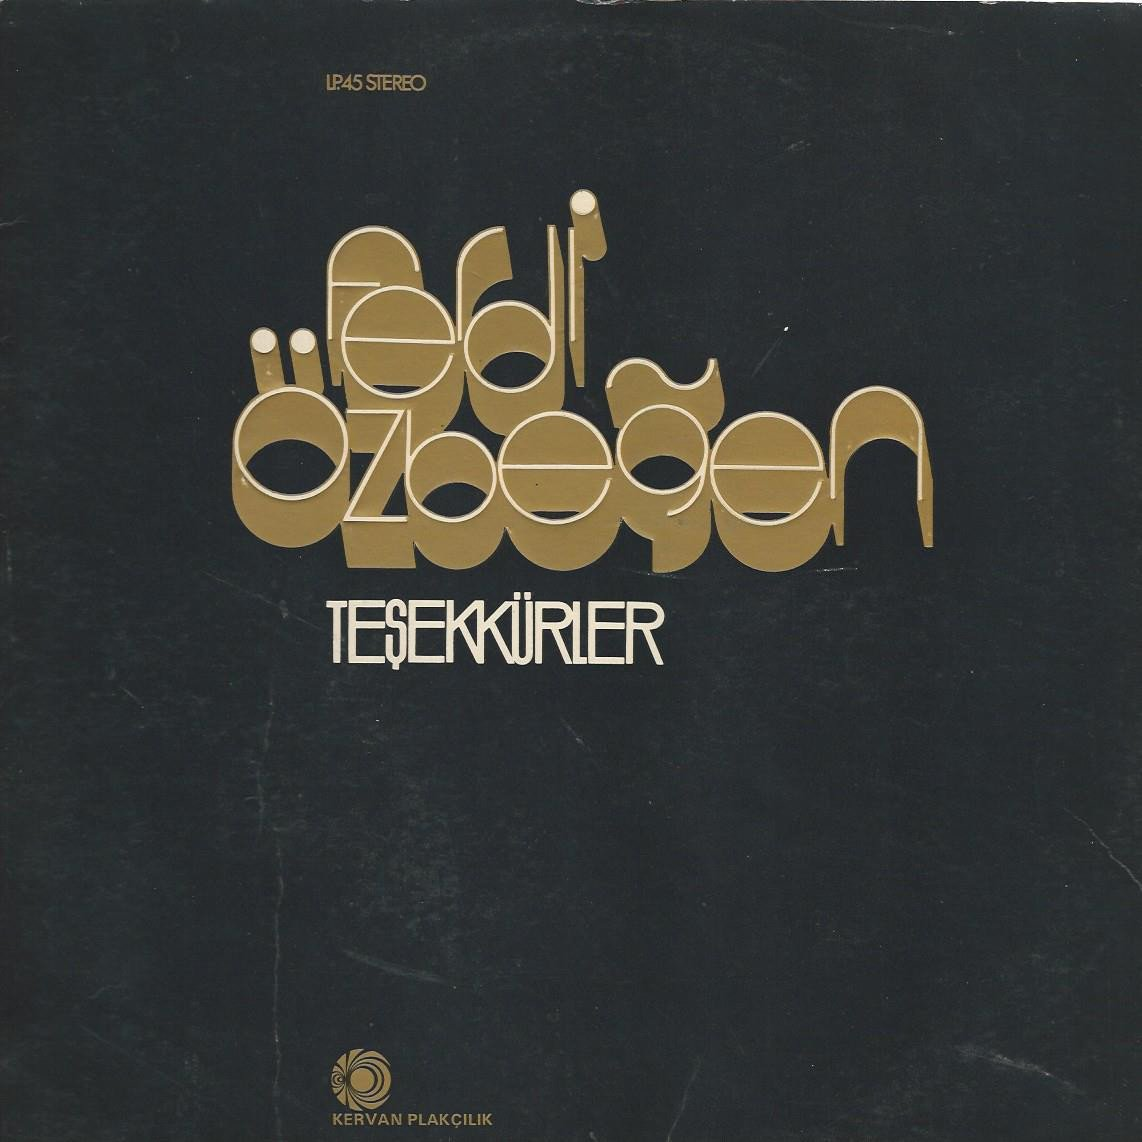
\includegraphics[height = 6\baselineskip]{./../01-solution/src.jpeg}
						\caption{}
						\label{subfig:01-01-src}
					\end{subfigure}%
					\begin{subfigure}{0.5\textwidth}
						\centering
						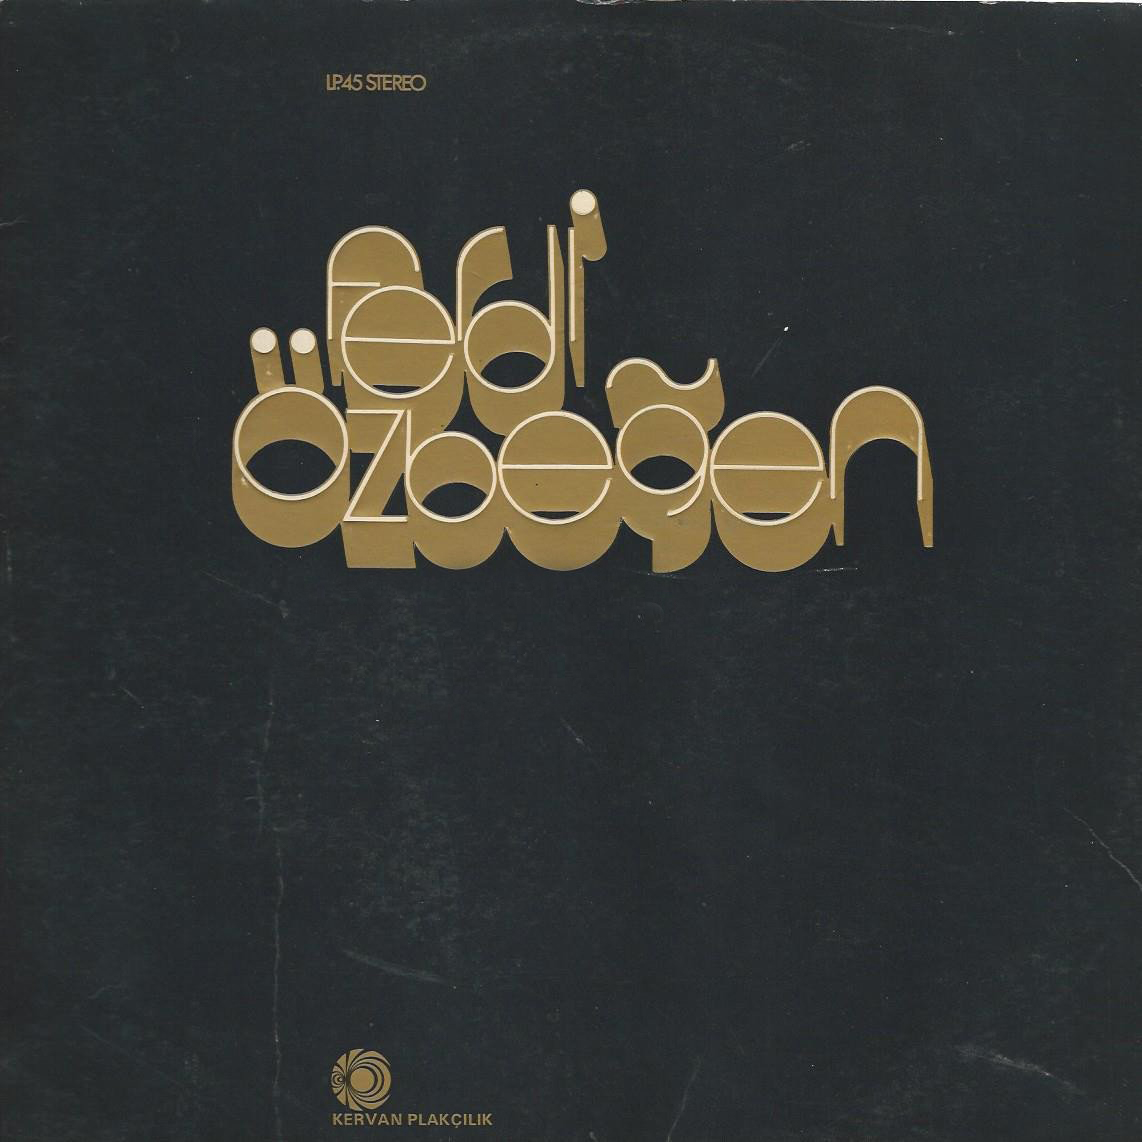
\includegraphics[height = 6\baselineskip]{./../01-solution/y03s01-multimedia-lab-02-01-p01-clone-stamp.jpg}
						\caption{}
						\label{subfig:01-02-res}
					\end{subfigure}
					\caption{Видалення елементів зображення за~допомогою інструмента~\emph{\textenglish{Clone Stamp}}}
					\label{fig:01-removal-clone-stamp}
				\end{figure}

			\subsubsection{За допомогою інструмента \emph{\textenglish{Patch Tool}}}
				Видаляємо елементи з~зображення за~допомогою інструмента~\emph{\textenglish{Patch Tool}}. Для~цього виділяємо область, з~якої необхідно видалити елемент, будь-яким зручним інструментом виділення, обираємо інструмент~\emph{\textenglish{Patch Tool}} та~пересуваємо виділену область до~тих пір, поки необхідний об'єкт не~буде видалений~(рис.~\ref{fig:01-removal-clone-stamp}).

				\begin{figure}[!htbp]
					\centering
					\begin{subfigure}{0.5\textwidth}
						\centering
						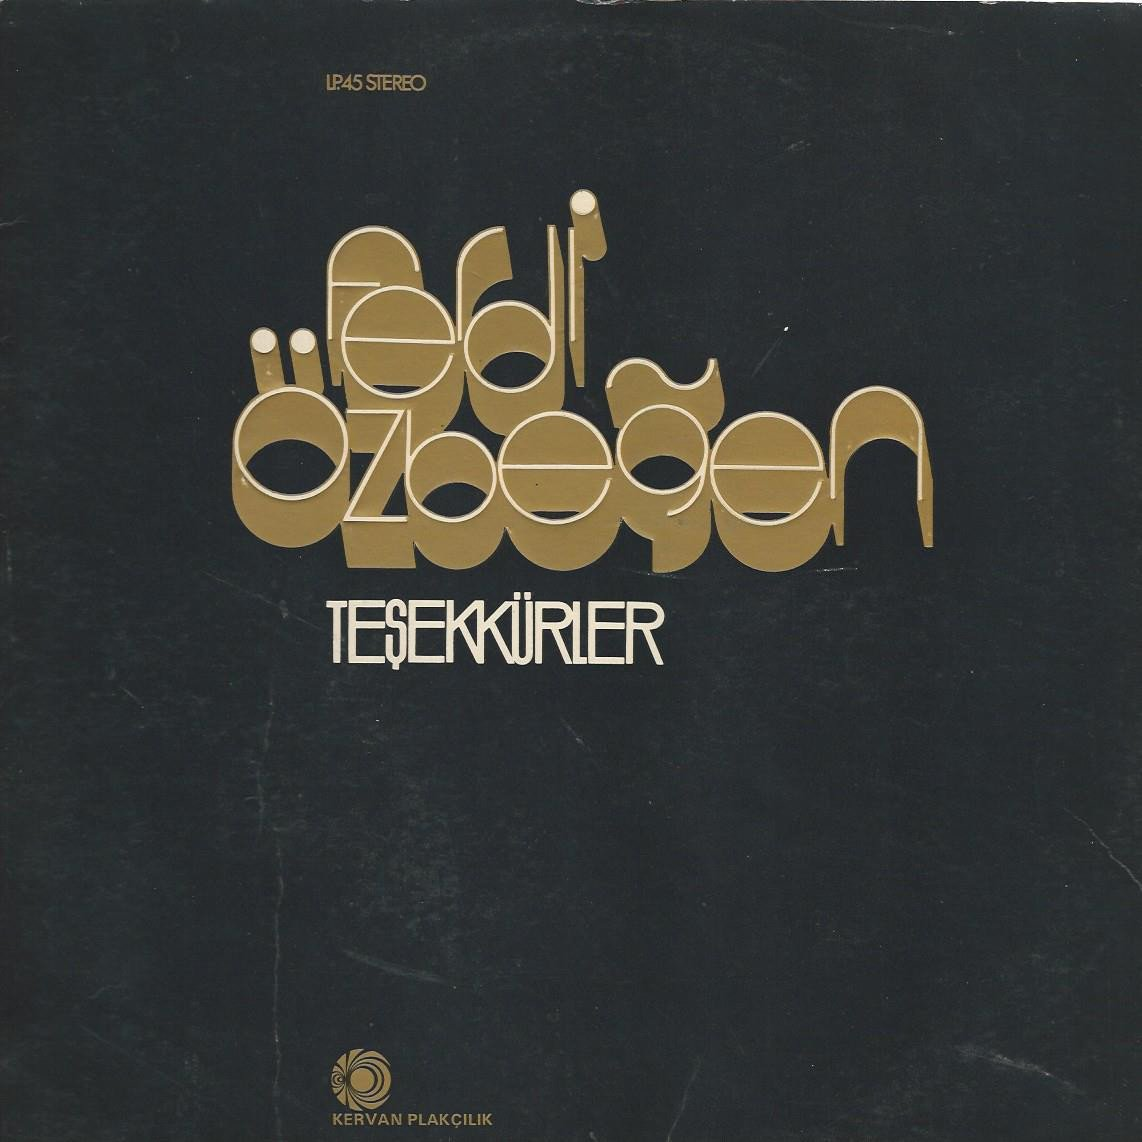
\includegraphics[height = 6\baselineskip]{./../01-solution/src.jpeg}
						\caption{}
						\label{subfig:02-01-src}
					\end{subfigure}%
					\begin{subfigure}{0.5\textwidth}
						\centering
						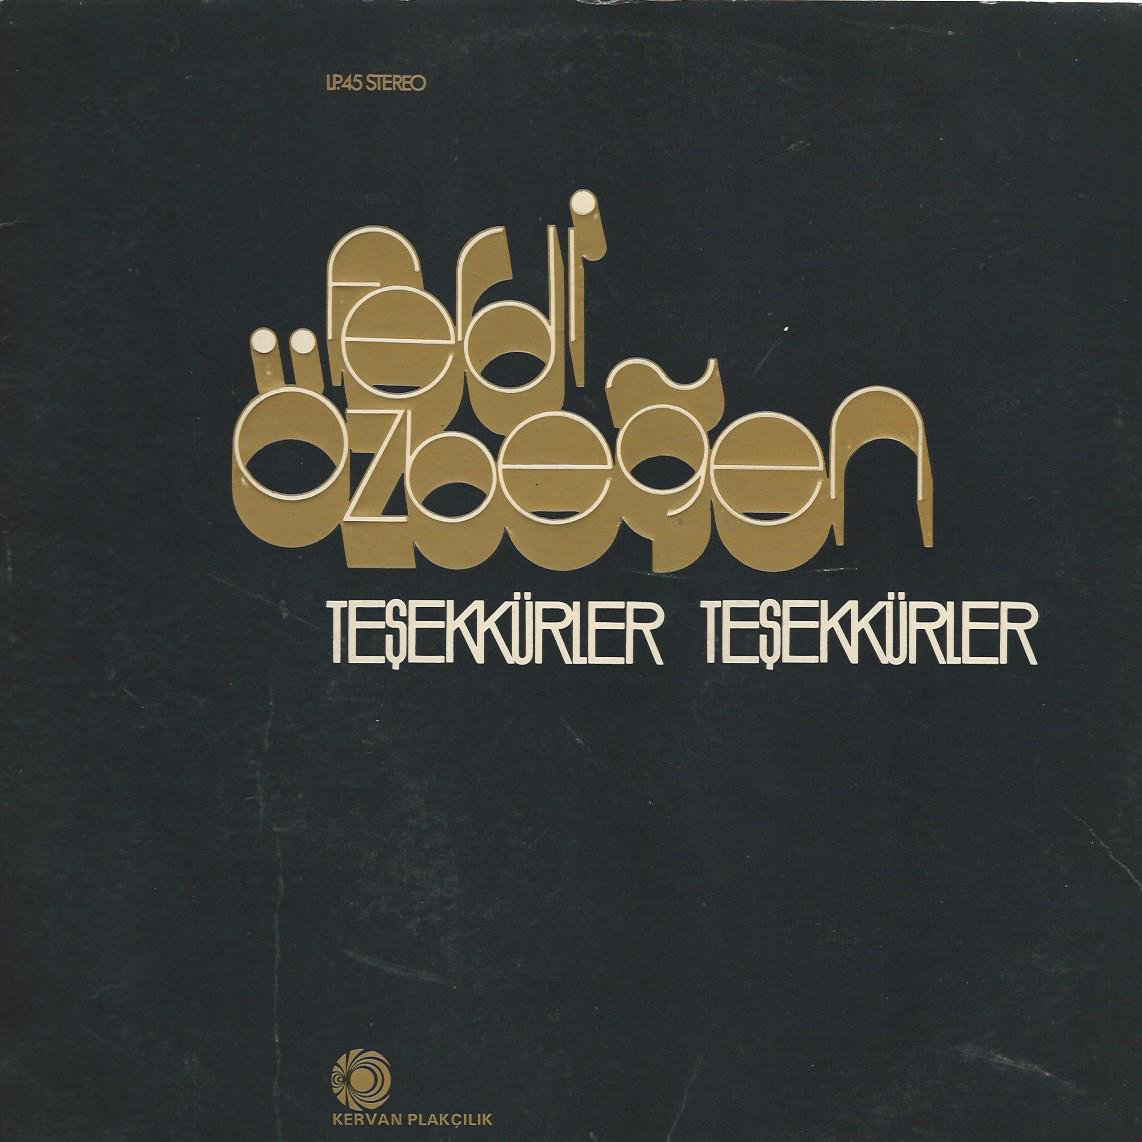
\includegraphics[height = 6\baselineskip]{./../01-solution/y03s01-multimedia-lab-02-01-p02-patch-tool.jpg}
						\caption{}
						\label{subfig:02-02-res}
					\end{subfigure}
					\caption{Видалення елементів зображення за~допомогою інструмента~\emph{\textenglish{Patch Tool}}}
					\label{fig:02-removal-patch-tool}
				\end{figure}

		\subsection{Відновлення відсутніх елементів~зображення}
			\subsubsection{За допомогою інструмента \emph{\textenglish{Clone Stamp}}}
				Відновлюємо відсутні елементи з~зображення за~допомогою інструмента~\emph{\textenglish{Clone Stamp}}. Для~цього обираємо і~налаштовуємо цей інструмент. Щоб налаштувати інструмент~\emph{\textenglish{Clone Stamp}}, необхідно обрати область, з~якої будемо клонувати зображення, для~чого натискаємо і~тримаємо натиснутою клавішу~\keys{\textenglish{Alt}}, наводимо курсор на~бажану область і~натискаємо ліву клавішу миші. Тепер, коли область, з~якої буде братись зображення, вибрана, відновлюємо необхідний елемент~(рис.~\ref{fig:01-removal-clone-stamp}).

				\begin{figure}[!htbp]
					\centering
					\begin{subfigure}{0.5\textwidth}
						\centering
						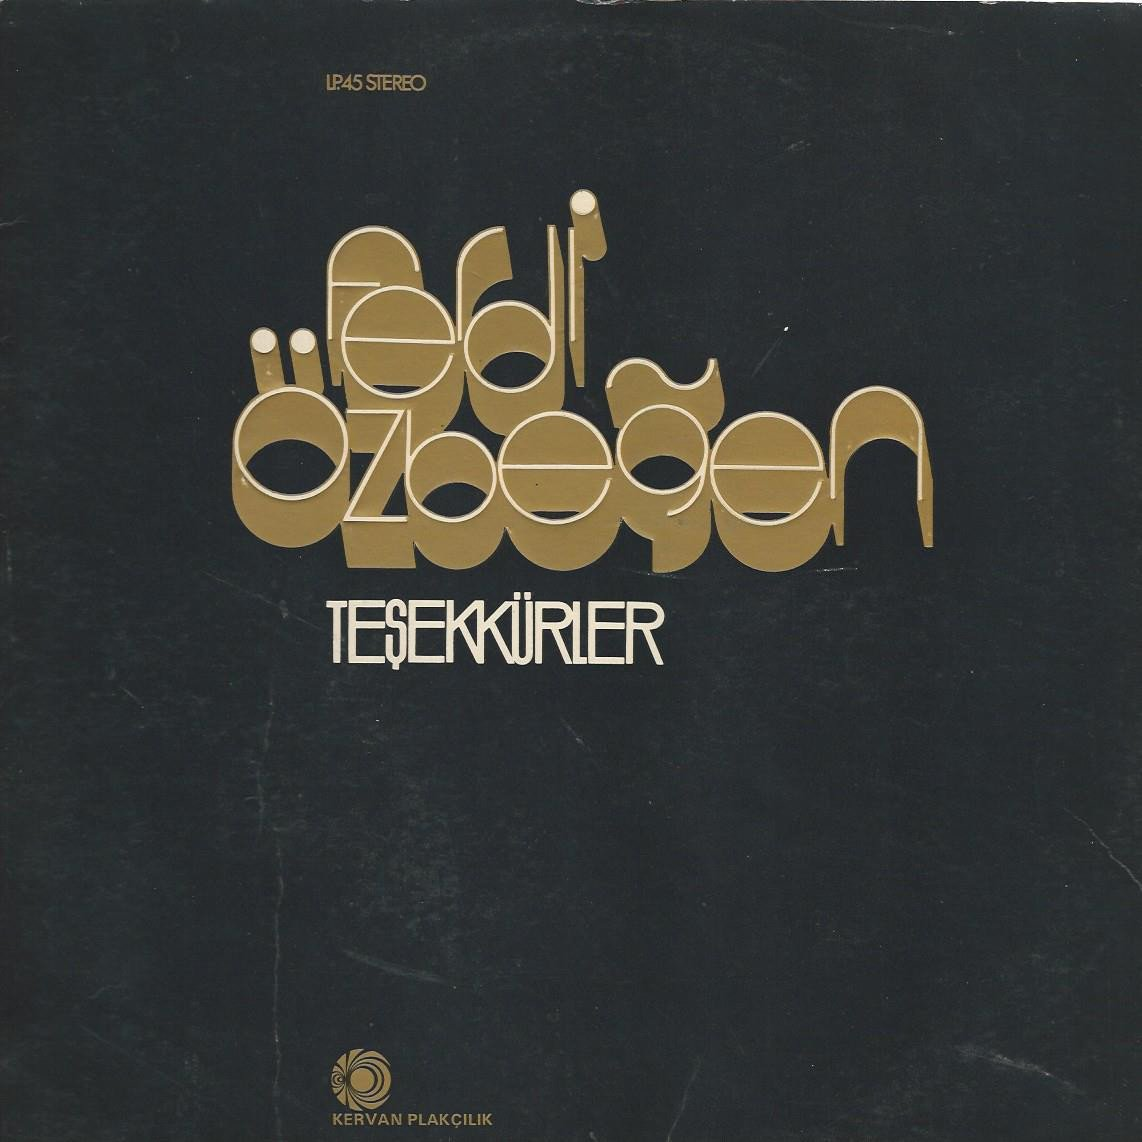
\includegraphics[height = 6\baselineskip]{./../01-solution/src.jpeg}
						\caption{}
						\label{subfig:03-01-src}
					\end{subfigure}%
					\begin{subfigure}{0.5\textwidth}
						\centering
						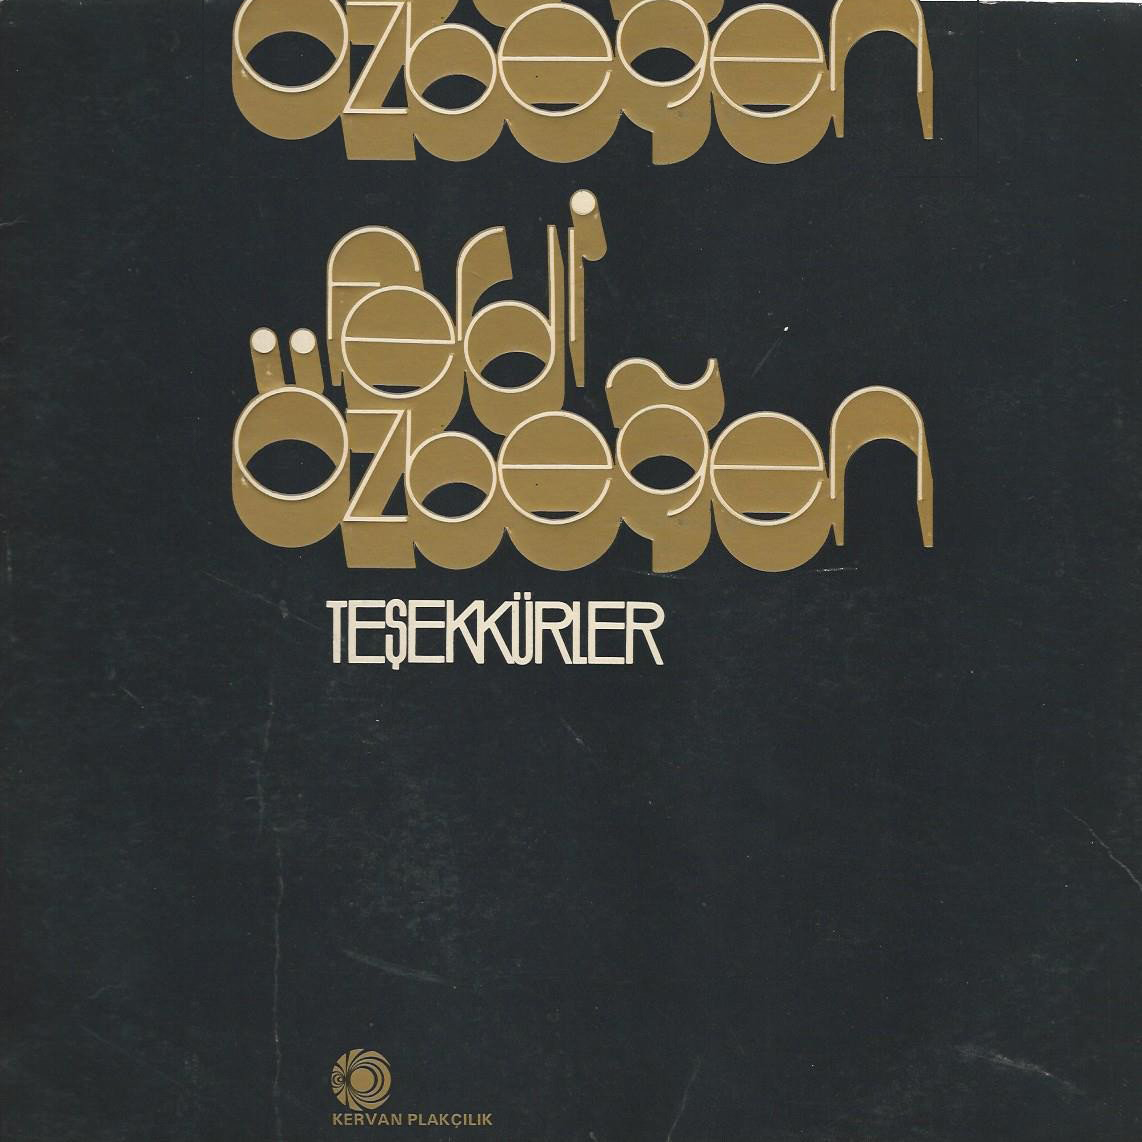
\includegraphics[height = 6\baselineskip]{./../01-solution/y03s01-multimedia-lab-02-01-p03-clone-stamp.jpg}
						\caption{}
						\label{subfig:03-02-res}
					\end{subfigure}
					\caption{Відновлення відсутніх елементів зображення за~допомогою інструмента~\emph{\textenglish{Clone Stamp}}}
					\label{fig:03-addition-clone-stamp}
				\end{figure}

			\subsubsection{За допомогою інструмента \emph{\textenglish{Patch Tool}}}
				Відновлюємо елементи з~зображення за~допомогою інструмента~\emph{\textenglish{Patch Tool}}. Для~цього виділяємо елемент, який необхідно відновити, будь-яким зручним інструментом виділення, обираємо інструмент~\emph{\textenglish{Patch Tool}}, перемикаємо режим роботи на~\emph{\textenglish{Destination}} та~пересуваємо виділений елемент в~цільову область~(рис.~\ref{fig:01-removal-clone-stamp}).

				\begin{figure}[!htbp]
					\centering
					\begin{subfigure}{0.5\textwidth}
						\centering
						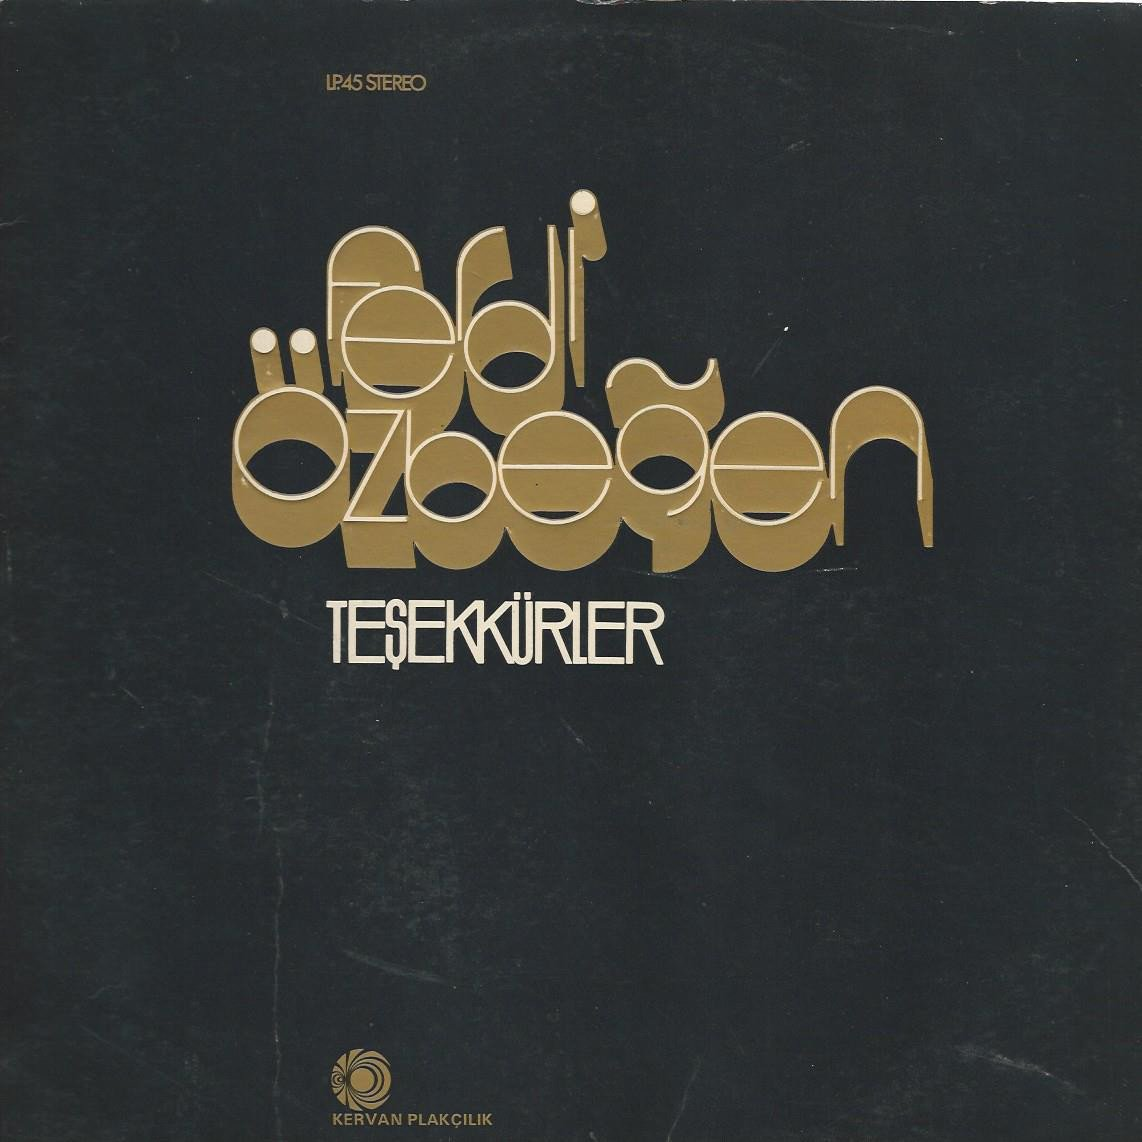
\includegraphics[height = 6\baselineskip]{./../01-solution/src.jpeg}
						\caption{}
						\label{subfig:04-01-src}
					\end{subfigure}%
					\begin{subfigure}{0.5\textwidth}
						\centering
						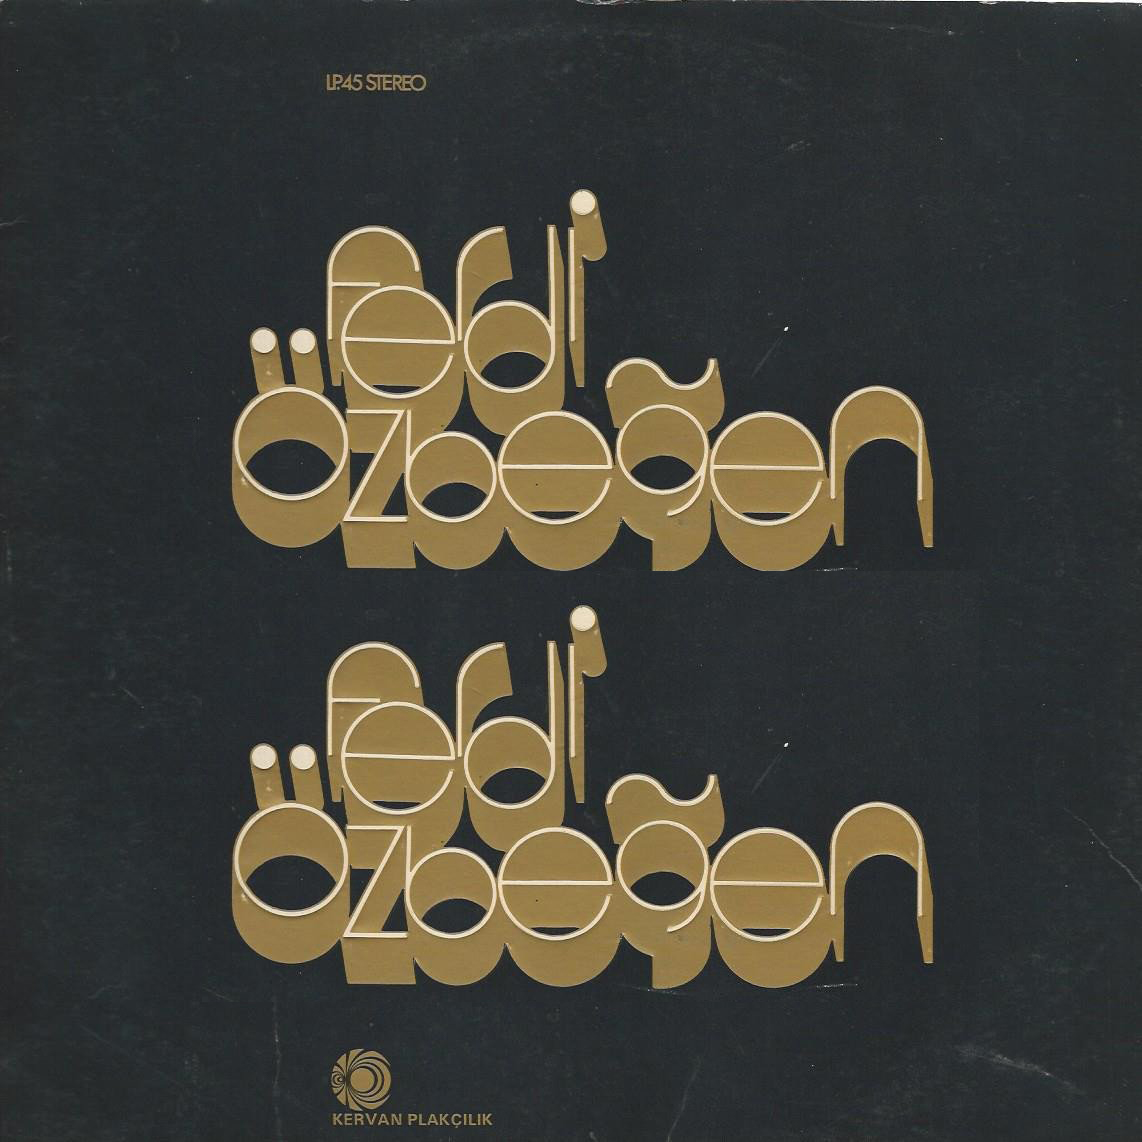
\includegraphics[height = 6\baselineskip]{./../01-solution/y03s01-multimedia-lab-02-01-p04-patch-tool.jpg}
						\caption{}
						\label{subfig:04-02-res}
					\end{subfigure}
					\caption{Відновлення відсутніх елементів зображення за~допомогою інструмента~\emph{\textenglish{Patch Tool}}}
					\label{fig:04-addition-patch-tool}
				\end{figure}

	\section{Висновок}
		Виконуючи дану лабораторну роботу ми~вивчили можливості і~ознайомились з~основними інструментами~\textenglish{Adobe Photoshop} для~ретушування зображень.

\end{document}
